\chapter{引言}
\rhead{引言}
\section{研究背景和意义}

由于生物实验的局限性,传统的微生物基因组学经常关注于单个人的细菌基因组。然而,环境中的微生物基因组通常会互相产生影响。
例如,人类中的微生物已被证明与常见疾病有关
如炎性肠病(IBD)的[1]和胃肠紊乱[2]。
宏基因组学(环境基因组学或生态基因组学)是直接从环境样本,例如人体肠道,土壤,空气中的尘埃中直接研究遗传物的学科。快速发展
随着新一代测序(NGS)技术的快速发展,我们可以直接对混合环境的DNA样品获得的多个物种进行测序。
宏基因组序列来自多个微生物基因组,并且通常
大多数宏基因组序列所在的物种名是未知的。
宏基因组分析的关键步骤就是将同一物种的DNA片段聚在一起。
这个任务被称为宏基因组序列的归类[3]。迄今为止,研究人员已经提出了大量的计算方法来解决这个问题。这些方法可以粗略的归为两类:
基于相似度和基于组成成分。

基于相似度的方法首先将元基因组序列比对到已知的基因组,然后根据比对结构进行归类。其中一个典型的方法是MEGAN[4].

显然,如果没有已知的微生物基因组,这个方法不能用。基于组成成分的方法通常采用
监督技术 将序列分配到不同的组。特征是直接从核苷酸序列从抽取的,包括寡核苷酸的频率
GC含量,密码子的使用等等。到现在为止,SVM [5],朴素贝叶斯[6],KNN [7],Interpolated 马尔可夫模型[8]等已经被用来对宏基因组序列进行归类。然而这些方法的性能仍然在很大程度上依赖于作为训练样本的基因组。
为了克服这些方法的缺点以上,无监督或半
监管技术提出了应对来自未知的宏基因组数据
种。 Wu等人[9]提出了一种称为AbundanceBin方法提取K-聚体
从序列读数和箱读取基于其k个聚体的覆盖率,其可以
独立的读取非常不同的丰度。然而,AbundanceBin不
正常工作时,该数据集包括读取相同的丰度。 Leung等
人。 [10]开发了使用4聚物打造的特征元簇3.0方法
向量。它读成许多小群的K-位数algo-第一组
rithm,然后合并小簇,以较大的,使得从序列的物种
低丰度的比率可被分成分离簇。元簇3.0 outper-
形式AbundanceBin上都均匀分布不均的数据集读取
的1000bp。后来,Wang等人元簇的推出了两款改进型
3.0,这是元簇4.0 [11]和元簇5.0 [12],为目的
处理短读。元簇4.0可与短处理读取小于500bp的
首先串联短读取到更长的基于序列重叠。
但是,它不能读取斌低丰度。元簇是5.0的扩展
元簇4.0搬运读取低丰度。近日,王某等人。人员开发
OPED元簇-TA [13],一个装配辅助分级的基于注释工具
分类注释读取。它装配读入长“的虚拟重叠群”,并
然后应用像元簇5.0的方法来聚类这些重叠群和读取,
最后分配产生的所有集群分类法。该系列的元簇
算法可以自动确定簇的数目,这是非常
对于宏基因组的分级重要内容大部分样本都来自不明
种真实数据。

\begin{figure}
\centering
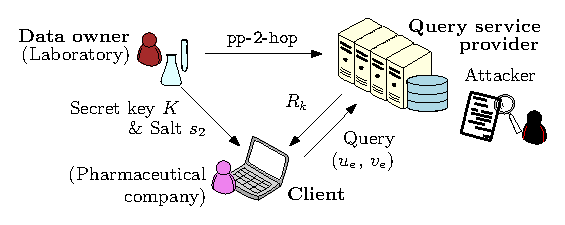
\includegraphics[height=4cm ,width=10cm]{example/system.eps}
%\vspace{-2ex}
\caption{系统模型概要}
\label{fig:overview}
\end{figure}


考虑图~\ref{fig:overview}中的一个例子,有一家制药公司,它主要的收入都来自于研发一些保健产品。这家公司可能刚刚发现了一种新产品的制药配方。为了节省做实验的人力成本,它常常需要去一个非常庞大的公开生物信息网络(例如\cite{biology})中去查询这些混合物的信息,以了解这些混合物之间的相互作用关系(可能是通过判断两种混合物在这个生物信息的网络上是否通过一定的化学作用可以转化,这就是一种可达性查询),判断这样一个混合物是否可以通过一定的生物酶的作用从另外一种或者几种化合物转化而来。然而从公司的角度来说,他们并不希望\SP 知道他们的查询内容,因为这可能涉及到知识产权问题,同时他们也不希望他们的竞争对手知道他们的查询内容。作为生物信息图数据的拥有者,他们一方面缺乏维护这样一个查询服务的经验,可能只有将数据通过一定的处理外包给一些专业的IT公司\cite{commercial}或者一些云计算平台(例如亚马逊AWS),利用这些平台庞大的处理查询请求的计算能力为他们提供查询服务;另外一方面,他们不希望将他们拥有的数据曝光给未授权的一些机构或者个人。作为一种折中的解决方案,他们可能只希望将数据的查询权限授权给一些购买了他们服务的用户。因此,防止\SP 获取客户端查询内容,或者通过推理得出图数据库的原始结构是一件非常具有挑战性的工作。

再考虑另外一个例子,在社交网络中,人与人可能通过电话的方式进行联系,我们可以用图中的一个顶点表示一个人,点与点之间的边表示人们有过电话的联系。考虑在一个刑事案件的侦破早期,警察可能要对一个犯罪嫌疑人进行调查,他们想知道都有谁和这个犯罪嫌疑人有联系,那么警察会向移动通信服务商提出查询请求。但是移动通信服务商可能不希望自己去维护这样的查询服务,所以他可能将他们的通信网络数据外包给一个查询服务提供商\SP 为其提供查询服务。但是,在外包给查询服务商的时候,由于这样的通信网络中有很多的敏感性的信息,所以移动通信服务商不希望查询服务提供商\SP 能够获得这个通信网络的结构信息。 同时,警察也不希望他们的查询内容和查询的结果被\SP 知道,因为这很有可能会暴露他们的侦查工作。在这种情况下,提供一种隐私保护的可达性查询服务变得非常迫切。



\section{研究内容和研究成果}

在本文中,我们的主要研究问题是:在查询服务提供商\SP 并不能被安全信任的情况下,针对图数据的拥有者如何保护其外包给服务提供商的原始数据结构信息;%作为图数据的拥有者如何对外包到服务商上的数据索引进行处理,使得\SP 不能够从索引中推理获取到原始图数据的结构信息,
针对查询服务的使用者,如何保护其发送给服务提供商的查询内容不被\SP 获取。根据我们已有的知识来看,目前还没有关于这一问题的相关研究。

%在论文中,我们的主要研究问题是在一个可达性查询服务中,如何使得可以得到我们想要的查询结果,同时使得具有不可信任性的\SP 不知道查询的顶点以及使得它不能够通过对密文的推理和通过索引的大小推理出图的结构信息。根据我们目前的知识来看,目前还没有这一方面的任何研究。

当前在学术界有很多关于高效的图数据上可达性查询算法的研究成果\cite{byron,pathhop,sigmod2013,chengjf2,pathtree,3hop,hopi,ferrari,gripp,bitcompression,grail,chen2008efficient,fan2011adding,yu2010graph,jin2008efficiently}。 在\cite{sigmod2012}中,作者将图上可达性查询的算法分为三类,分别为基于传递闭包压缩的索引算法、优化的在线搜索查询算法和基于hop的索引算法。这三类算法中,第一类通常具有高昂的存储开销,对于部分大的图数据,这种方法可能无法工作;第二类算法由于需要在线的搜索,通常具有较慢的查询速度;第三类算法通常查询时间和索引大小介于以上两者之间。在第二章中我们将详细讨论各类算法的特点。在本文中,我们提出了基于2-hop的索引算法\cite{cohen}对可达性查询进行隐私保护。采用2-hop的索引方法来实现隐私保护的可达性查询算法主要有以下三方面的优势:第一、2-hop索引的结构非常简单。在2-hop索引中,图中的每个顶点$u$与其他顶点之间的可达性关系都通过两个集合($\lin(u)$和$\lout(u)$)来表示。即在2-hop索引中,对于图中的每个顶点$u$我们都使用两个集合$\lin(u)$ 和$\lout(u)$来表示顶点$u$与图中其他顶点之间的可达性关系。第二、基于2-hop 索引的可达性查询算法很精巧与简单,要判断两个顶点($u$,$v$)是否可达,我们只需要做一个简单的交集运算就可以判断两个顶点是否可达。正是这样简单的索引结构和精巧的可达性查询算法使得在做可达性查询的同时保护隐私成为了可能。第三、在学术界,2-hop索引方法仍然是一个非常热门的索引算法。在2-hop索引算法基础上,关于大图分割\cite{chengjf2}、 索引压缩算法\cite{chengjf1}和索引更新算法\cite{byron,hopi}这些方面的研究成果可以很容易的应用到我们的隐私保护可达性查询算法上。

在本文中,针对一般的图数据,在2-hop索引算法的基础上,我们提出了\pphop (隐私保护的2-hop算法)。该算法主要思想是在2-hop的查询算法中,要判断两个顶点是否可达,仅仅需要在两个中心顶点集合之间做一个交集操作。基于以上的查询算法流程,在建立索引时,我们通过相应的启发式算法使得所有可能的两个集合之间的交集结果尽可能小,同时通过在每个顶点的$\lin$ 和$\lout$ 集合中加入最少的人工代理中心点使得任何两个集合之间的交集大小相同。这一步的意义在于,对于任何查询,在\SP 看来,他们查询得到的交集大小完全一致,以避免不同交集大小带来的信息泄露。然后同时通过相应的算是使得建立出来的每个点的$\lin$,$\lout$的集合大小也在一个用户指定的差值范围内。在前面建立好的索引的基础上,我们再通过对索引进行加密操作,然后提出了基于索引密文的可达性查询算法,同时,我们对这样的一个隐私保护的2-hop索引方法进行隐私保护证明。

针对稀疏图,我们提出了另一种基于2-hop的索引算法\ppmuihop ,在该算法中,我们通过算法保证图中各个顶点之间的2-hop索引交集大小始终为1。这样做的好处在于:对于稀疏图,图中只有极少的顶点之间是可达的,所以如果要使图中任意两个顶点的2-hop交集结果都为大于1的集合,我们需要引入较多的人工代理中心点来实现隐私保护的目的,但是如果使得所有的交集大小为1,可以在保证安全特性的前提下,大幅度的减少索引的大小。

本文中,我们的对于可达性查询的隐私保护问题的主要贡献可以总结为以下六点:
\begin{itemize}
\item 我们设计一种新的建立2-hop索引的启发式函数,使用该函数建立的2-hop索引能够保证任何两个顶点之间的索引交集大小较小,同时也能使得全局的2-hop 索引大小最小。
\item 我们提出了两种人工代理中心点添加算法,使得图中每个顶点的2-hop索引具有相同的大小,同时使得所有可能查询的查询结果具有相同的交集大小。
\item 我们提出了一种可达性查询的隐私保护索引结构\pphop ,该索引可以保证原始图数据数据结构和可达性查询结果的安全性。
\item 我们提出了在密文索引环境下的可达性查询算法,并对其优化,提出了一种基于乘法同态加密的优化查询算法。
\item 针对稀疏图的特殊性,我们提出了另一种高效的隐私保护可达性索引方法\ppmuihop 。
\item 从理论上和实验上,我们证明了两种可达性查询隐私保护算法的高效性和可扩展性。
\end{itemize}


\section{本文结构}
本文的组织结构如下:在第二章中我们介绍目前在图可达性查询领域的一些相关工作。在第三章中,将介绍本文算法的背景知识、问题定义和解决方法的概要介绍。在第四章中,我们提出了\pphop 索引建立算法,索引优化算法和查询流程优化,并通过实验对我们的索引方法及其查询效率进行验证。在第五章中,我们针对稀疏图提出了一种更加优化的\ppmuihop 索引方法,并通过实验,对该算法在稀疏图上的数据特性进行分析。在第六章中,我们对本文进行总结,并对将来可以进一步改进的方向进行展望。
